\chapter{Classification Rule Learning} \label{chap:rule}

Rule learning can be used in a supervised manner for classification, or in an unsupervised manner for knowledge discovery \cite{agrawal1996fast} \cite{kavvsek2006apriori}. In this work, rule learning is used for classification but takes cues from the other contexts.

This chapter will examine the individual parts of a rule learning system and present a popular implementation of classification rule learning. Section \ref{chap:rule:back} will provide an introduction to the architecture of a rule learning system.
Section \ref{chap:rule:ripper} will use this architecture to introduce the RIPPER classification rule learner, which is perhaps the most famous rule learner. 
The specifics of the rule learning system used in this work will be detailed in Chapter \ref{chap:algo}.
This chapter provides a basic introduction into each section of classification rule learning, for a more in-depth introduction please see \cite{furnkranz2012foundations}.


\section{Background} \label{chap:rule:back}

The standard unit of rule learning is the \emph{rule}. A rule is an unordered combination of binary features that together restrict a population to a select few individuals that match each feature in the rule. A feature is a binary test that can be applied to the attribute matrix $A$ (defined in Section \ref{chap:data:layout}) that will categorize each client as "matching" the feature, or not.
As such, each attribute matrix will have a distinct set of features.
The set of all features will be denoted $\mathcal{F}$ where $\mathcal{F} = \{ f_1, f_2, ..., f_{|\mathcal{F}|}\}$, $f_i$ is the $i$th feature, and $|\mathcal{F}|$ is the size of the set $\mathcal{F}$.
A typical feature in this work, will look like $a > 30$ where $a$ is an attribute in $A$, this feature would match all clients who have slept at the DI more than 30 times.
A single rule is typically denoted $c \leftarrow f_1 \land  f_2 \land ... \land f_L$ where $c$ is the assigned class label (chronic/not chronic in this work) and $L$ is the rule length. In this work, a simpler notation will be utilized that fits better with plain text and the fact that all rules in this work will assign the positive class. Rules will take the form $f_1$ AND $f_2$ AND $...$ AND $f_L$ where each feature will be represented by its actual value (i.e Sleep $>$ 30 AND Age $>$ 55).
The number of features in a rule is known as the rule length, or depth, this work will refer to both.
As more features are added to a rule, the population covered by the rule decreases in size (or stays the same). This is because a rule is the logical conjunction (intersection) of all of its features.

A rule set is the logical disjunction (union) of rules, meaning that as more rules are added to the rule set, the size of the covered population increases (or stays the same). Together, the rules and rule set present a powerful framework for classification, as the rules provide specific classifications that cover a relatively small population and the sets combine them to cover a wide population in a targeted way that more general rules can not duplicate.

% It is possible to consider an ordered rule set (that is, rules must be viewed in a certain order with order representing rule quality or some other metric), however, in this work only unordered rule sets will be considered (this work deals only with a single class, meaning there is no distinction between ordered and unordered rule sets)

There are four main sections of a rule learning system: feature generation, individual rule learning, rule set learning, and post-processing/pruning. 
Figure \ref{fig:covering} demonstrates the basic flow of the classification rule set learning. The feature generation phase is responsible for processing $A$ into a set of features, more details are found in Section \ref{chap:rule:pre}. The features in this set are combined by the rule learning to produce rules, Section \ref{chap:rule:individual} covers the details on how this could be done. The rule learner is repeatedly called by the rule set learner until some stopping condition is met, before that, the generated rules are added to the currently growing rule set. Section \ref{chap:rule:sets} has more details on rule set learning. The final stage, post-processing, performs some form of optimization on the generated rule set. A common technique is to "prune" the rules in the rule set. Pruning is a process in which features are iteratively removed from the rules in a rule set with the intention of improving the classification performance of the rule set. Details on this post-processing step/pruning are provided in Section \ref{chap:rule:post}.




\begin{figure}[h]
    \centering
    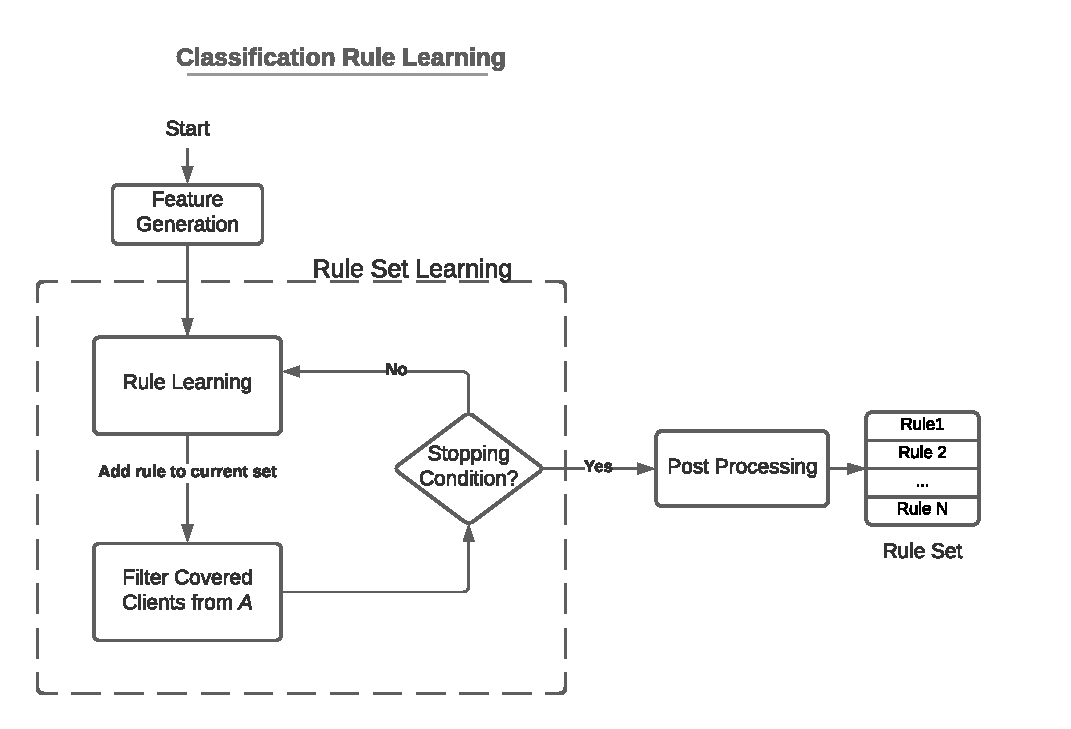
\includegraphics[width=1\textwidth]{Figures/Covering-Algorithm.pdf}
    \caption{A high-level overview of a classification rule learning system.}
		\label{fig:covering}
\end{figure}


\subsection{Feature Generation} \label{chap:rule:pre}

As features are typically descriptions of a data set (e.g Sleep $>$ 30), they will need to be derived somehow from the data. The general format of features also needs to be chosen by the system designer and will have an impact on the feature generation procedure. A common feature generation procedure is to take the range of each attribute and generate several "bins" based on this range. The bins can be evenly spaced, or the result of some clustering algorithm. The resulting "bins" will be used as features (e.g 25 $<$ Sleep $<$ 30). Another approach is to consider thresholds, which are the same as bins, but one side is unbounded (e.g. Sleep $>$ 24). More examples are provided in Table \ref{tbl:rule:examplefeatures}. Similarly, these threshold values can be evenly spaced, exponentially spaced, or based on some clustering or partitioning algorithm. 

A common problem with rule learning is that the space of all possible rules is large ($\sum_{k=1}^{|\mathcal{F}|} {|\mathcal{F}| \choose k}$), and many (if not most) rules are not useful. Due to the combinatorial nature of rules with respect to features, the complexity of the rule space increases exponentially with the number of features. The feature generation procedure needs to take this into account and generate a minimal set of features that can support high-quality rules. Additionally, this means there is much to be gained from removing features that are not useful before the learning process begins. There are many methods of determining the usefulness of a feature, but perhaps the two most common are pairwise correlation and feature coverage.

Pairwise correlation examines every available feature and builds a correlation matrix, that is, a matrix whose columns and rows are the set of all features, and whose values are the correlation between those features. The Pearson correlation coefficient \cite{benesty2009pearson} can be used to get these correlation values. A correlation threshold is then given and any pairs with a correlation higher than the threshold will be reduced to a single feature. One method of determining which feature in the pair should be removed is to take the sum of all correlations of the two features and discard the one with a larger total correlation. This pruning is then repeated on the reduced set of features until all pairs are below the given correlation threshold.

As noted above, each feature applied to $A$ generates a list of clients matching the feature. A features coverage is the number of positive individuals who match the feature (in this work, clients who are chronic or have the potential to become chronic are considered for coverage). A feature with low coverage can only produce rules with even lower coverage (as noted in Section \ref{chap:rule:back}, paragraph 1). This suggests that features with abnormally low coverage can be excluded from the rule learning procedure as they are unlikely to produce useful rules.
Another reason to trim low coverage rules is they can lead to over-fitting. Rules with low coverage are inherently over-fit as they target a small subset of the population which does not necessarily represent the broader chronic population.
In this work, low coverage is defined as having a Support $< 0.5\%$, which in this data set covers approximately 5 clients.

After this stage, the rule learning system will have a set $\mathcal{F}$ of available features. Table \ref{tbl:rule:examplefeatures} contains a list of example features using attribute names from Chapter \ref{chap:data}.


\begin{table}[h]
	\centering

	\begin{tabular}{c}
	\toprule
	Sleep $> 30$ \\
	Bar $\leq 1$ \\
	Log $= 15$ \\
	$55 \leq$ Age $< 79$ \\
	Log $> 15$  \\
	Sleep $\leq 30$ \\
	Bar $> 1$ \\
	EmployeeIsCounsellor $< 6$ \\
	Age $> 65$ \\
	CounsellorsNotes $> 16$ \\

	\bottomrule
	\end{tabular}

	\caption{Example features.}
	\label{tbl:rule:examplefeatures}
\end{table}


\subsection{Learning Individual Rules} \label{chap:rule:individual}
Within the context of rule learning, the user is often most interested in the best rule (or top $N$ rules) possible from a set of features $\mathcal{F}$. Best refers to a rule's ranking with some given quality metric. For example, a common quality metric is Accuracy, which measures the proportion of correct positive and negative classifications. See Appendix \ref{chap:perf} for an evaluation and discussion of different metrics.  Alternatively, a user might want a list of all rules sorted by some given quality metric. In both cases, a search algorithm must be employed that will discover the top rules.

In general, all of these search algorithms follow the same process. Initially, the search space is $\mathcal{F}$ and the initial rule is the default rule. The default rule being the class label that will be assigned to the examples that are not covered by the rule set. In binary classification systems such as this, the default rule has no features and results in a negative classification (not chronic in this work). Using Table \ref{tbl:rule:examplefeatures} as $\mathcal{F}$, a rule learner would begin the learning process by selecting one feature randomly (typically the first feature in the set). For example, the Sleep $> 30$ feature could be added to the current rule. The next step will be determined by the exact search algorithm used.

The simplest of these search algorithms would be breadth-first search (BFS) and depth-first search (DFS). Both of these algorithms are examples of exhaustive search and will discover all rules within a bounded search space. The only difference is the order in which rules are discovered.

BFS is an iterative algorithm that searches all rules made up of only a single feature, before searching all rules made up of two features, and so on. Continuing from the above example, the BFS algorithm will create a set of rules from Sleep $> 30$ and the remaining features in $\mathcal{F}$, (e.g. Sleep $> 30$ AND Bar $\leq 1$, Sleep $> 30$ AND Log $= 15$, etc.) producing $|\mathcal{F}| - 1$ new rules. For each rule in this resulting rule set, the above procedure will be duplicated, that is, each rule that was just added to the rule set will produce $|\mathcal{F}| -2$ new rules. This procedure is repeated until all possible rules are created from $\mathcal{F}$. The rules can now be ranked by a quality metric (e.g. Accuracy) and the best rule (or best $n$ rules) can be returned.

DFS recursively searches the space of all possible rules and adds features to the current rule until there are no more available features, or some other stopping condition is met. This is conceptually the same as BFS, but the order of rule generation is different. Starting again with one rule, Sleep $> 30$, the DFS algorithm will create the next rule by adding a feature from $\mathcal{F}$, for example, Sleep $> 30$ AND Bar $\leq 1$. The next step will add a feature to the current rule, for example, Sleep $> 30$ AND Bar $\leq 1$ AND Log $=15$. The algorithm will continue adding one feature at a time until $\mathcal{F}$ is empty, at which point it will backtrack and substitute one feature for another. For example, at one stage in the algorithm, the rule Sleep $> 30$ AND Log $= 15$ will be generated. The generated rules will be identical to the BFS algorithm, hence they are both exhaustive search techniques. The difference between these techniques becomes apparent when stopping conditions aside from $|\mathcal{F}| = 0$ are used, as this is when rule set ordering can become relevant.

It is common to use a given depth as a stopping condition, as in, only rules up to a certain depth will be created. Another common stopping condition is to supply a given rule quality measure and set a minimum value for the measure. While these simple search algorithms are quite powerful, the entire search space of all possible rules is often large enough that it can be infeasible to search beyond a depth of 2 or 3.
Along with limits on search depth, exhaustive search techniques can suffer from over-searching \cite{quinlan1995oversearching} \cite{janssen2008oversearching}. That is, the ability to search over all possible rules can result in a rule learning system that over-fits the data and will not generalize well.
 Fortunately, there are heuristics that can be used to reduce the search space and help prevent over-searching.

 The Apriori algorithm \cite{agrawal1996fast} is most famously used in the field of association rule learning, but has also been adapted for use in classification rule learning \cite{liu1998integrating} \cite{liu2000improving} \cite{jovanoski2001classification}.The Apriori algorithm is a heuristic search based on BFS. The algorithm differs from BFS by evaluating each generated rule and discarding all rules that fall below a given quality threshold. This heuristic limits the search space thus allowing for more efficient discovery of rules. The quality measures used are Support, Confidence, and Lift. These measures are precisely defined in Appendix \ref{chap:perf}, but for now, it is enough to know that Support is equivalent to the coverage of a rule, Confidence is the conditional probability of a true positive, and Lift represents the improvement of Confidence relative to a random guess. If a generated rule is below the given Support it will be removed from consideration. This effectively reduces the severity of over-searching by reducing the search space of the algorithm (which removes the guarantee of a global optimum). Using Support in this way performs the same role as the coverage feature-filtering technique in Section \ref{chap:rule:pre}. After the rules have been generated, all the rules are sorted by Lift, and any rule with Lift less than 1 is removed. These are rules that do not provide additional Confidence beyond a random guess.

 Hill climbing is an alternative type of rule search algorithm, which follows a DFS approach, allowing it to discover much longer rules. The difference is that hill climbing will only follow a single path (it is not exhaustive). Hill climbing starts with the set of all features and selects the "best" feature, based on some provided quality measure. This feature is added to the current rule, and the procedure is repeated, $|\mathcal{F}|-1$ new rules are generated by adding a feature to the current rule and the "best" rule is selected. This procedure is repeated until some stopping condition is met. This condition can be the same as above (maximum depth) or something specific to hill climbing such as stopping when the quality difference between the current rule and the previous falls below a given threshold. The difference between hill climbing and DFS is hill climbing adds features based on which current feature will produce the best rule, and hill climbing never backtracks. This makes hill climbing very efficient because it does not generate all possible rules.
Unfortunately, hill climbing suffers from myopia by following the current optimal path and can thus miss a globally optimal rule that has a non-optimal predecessor.

Beam search is an improvement on hill climbing that maintains a "beam" of the $b$ best rules and will generate the set of potential rules by extending the $b$ best rules. The hill climbing procedure is simply the beam search with a beam size of $b=1$. Similarly, DFS is a beam search with $b=|\mathcal{F}|$. This alleviates the problem somewhat by allowing for an expanded search space but does not guarantee a globally optimal solution.

% This stage will generate a rule made up of one or more features. Table \ref{tbl:rule:examplerules} demonstrates a set of fabricated rules, made up of features from Table \ref{tbl:rule:examplefeatures}.


% \begin{table}[h]
% 	\centering

% 	\begin{tabular}{c}
% 	\toprule
% 	Sleep $> 30$ AND Bar $\leq 1$ \\
% 	Sleep $> 30$ AND Log $= 15$ \\
% 	Bar $\leq 1$ AND Age $> 65$ AND Sleep $\leq 30$ \\
% 	Log $> 15 10$ AND CounsellorsNotes $> 16$ \\
% 	Log $= 15$ AND Sleep $> 30$ AND Bar $> 1$ \\
% 	CounsellorsNotes $> 16$ AND EmployeeIsCounsellor $< 6$ AND Bar $\leq 1$ \\

% 	\bottomrule
% 	\end{tabular}

% 	\caption{Example rule set.}
% 	\label{tbl:rule:examplerules}
% \end{table}

\subsection{Learning Rule Sets} \label{chap:rule:sets}
Just as with rule learning, rule set learning is another simple operation that can be performed in any way that the rule learning system designer sees fit. For example, the most basic rule set learning algorithm would be to take the top $N$ rules generated by the rule learning procedure. This is not an ideal approach as it does not examine the impact each rule has on the rule set and can produce significant overlap between rules. Slightly more complex than that is the commonly used Covering algorithm \cite{michalski1969covering}.

The Covering algorithm, as the name suggests, is primarily concerned with the effect a new rule will have on the population covered by a rule set. Specifically, the covering algorithm is a loop that has two main functions. First, it searches for the top rule in the set of all rules (using any rule search method). Second, it removes all individuals covered by that rule from the attribute table. These two operations are repeated, with the rule learning procedure using the new attribute table at each iteration, and each rule learned being added to the current rule set. The loop stops when a given stopping condition is reached.
The stopping condition is typically when there are no more available rules, or when the rule set has 100\% coverage of the positive examples. This basic loop can perform fairly well but is often too eager in removing covered clients, which can impact the performance of rules generated later as they will have a much smaller database to draw from.

The weighted covering algorithm \cite{lavrac2004weighted} is a modification to the standard covering algorithm that assigns each client a weight. This weight is used by the top rule generating algorithm and corresponds to the degree a client should be considered by the rule learning procedure. Each time a client is covered by the top rule, this weight is reduced until a client is dropped entirely from consideration. The standard covering algorithm can be seen as a special case of the weighted covering algorithm, where a client is dropped from consideration after only being covered a single time. A simple method of calculating weights is the additive weighting scheme \cite{lavrac2004weighted} which is defined $weight = 1/(1+n)$ where $n$ is the number of times a client has been covered in the covering loop. The additive weighting scheme is recommended for experimental use in \cite{lavrac2004weighted}.

% After this stage, the rule learning system will have generated a rule set just like the one presented in Table \ref{tbl:rule:examplerules}. Note, there is not typically a limit to the number of rules in a rule set, the example in Table \ref{tbl:rule:examplerules} is fabricated.

\subsection{Post-Processing} \label{chap:rule:post}

The post-processing step can take place after rule set generation, or after the single rule procedure. It is used to compensate for possible over-fitting during the rule (set) learning procedure. Typically this is some form of pruning procedure (removing features from a rule). While there are several pruning procedures, such as Reduced Error Pruning \cite{brunk1991rep} or Reduced Error Regrowth \cite{cohen1993pruning}, a full examination of these methods will not take place in this work. Instead, a general introduction to the broad technique will take place.

The procedure for pruning proposed by Pagallo and Haussler \cite{pagallo1990pruning} is to split the data into a growing set $\mathcal{G}$ and a pruning set $\mathcal{H}$. These are similar to a training and testing set. The growing set $\mathcal{G}$ is used for the rule learning procedure, resulting in a set $\mathcal{R}$.
The rules in $\mathcal{R}$ then undergo the pruning process. The pruning process is a simple loop that removes one feature from one rule at a time. The rule set performance is then tested against $\mathcal{H}$ using either the same quality metric as was used in rule set learning, or a different one. If the prune successfully improves the rule set quality, it will be accepted and the pruning procedure will be repeated on $\mathcal{R}'$. The pruning procedure stops once additional prunes are unable to increase the quality of $\mathcal{R}'$. The pruning procedure is useful in combatting over-fitting by removing features that make rules overly specific (over-fit).

% Table \ref{tbl:rule:exampleprune} demonstrates a new rule set that might be generated after the rule set in Table \ref{tbl:rule:examplerules} was subjected to such a pruning procedure. Features highlighted in red are those that have been pruned by the pruner. In this (fabricated) example, the pruner has removed some redundant features and some features that did not improve the rule quality.


% \begin{table}[h]
% 	\centering

% 	\begin{tabular}{c}
% 	\toprule

% 	\prune{Sleep $> 20$ AND} Log $> 22$ \\
% 	Sleep $> 30$ AND Age $> 55$ \\
% 	\prune{Bar $\leq 1$ AND} Age $\geq 55$ AND Sleep $> 25$ \\
% 	Log $< 10$ AND CounsellorsNotes $< 5$ \\
% 	Log $< 3$ \prune{AND Sleep $> 15$} AND Bar $\geq 3$ \\
% 	CounsellorsNotes $> 16$ \prune{AND EmployeeIsCounsellor $>12$ AND Bar $\leq 1$} \\

% 	\bottomrule
% 	\end{tabular}

% 	\caption{Example rule set after pruning.}
% 	\label{tbl:rule:exampleprune}
% \end{table}

\section{RIPPER} \label{chap:rule:ripper}



\RIPPER (RIPPER) \cite{cohen1995ripper}, known by the popular JRIP, an implementation of RIPPER in the Java programming language included in the WEKA workbench \cite{frank2005jrip} is a highly regarded classification rule learning system. RIPPER was designed primarily to overcome the over-fitting issues described above and to improve the efficiency of its predecessor \IREP (IREP) \cite{frnkranz1994irep}. As such the broad structure of the RIPPER and the IREP algorithms are the same, only the RIPPER algorithm will be presented here. The reader is referred to \cite{frnkranz1994irep} for more information on IREP. The following sections will break the RIPPER algorithm into four sections of classification rule learning, feature generation, rule learning, rule set learning, and post-processing and detail each one.

\subsection{Feature Generation}
The RIPPER algorithm considers features of the form $a_n = v$ where $v$ is a value present in $a_n$ and $a_n$ is made up of integer values. For continuous attributes, RIPPER considers features of the form $a_c \leq \theta$ and $a_c \geq \theta$ where $\theta$ is a value present in attribute $a_c$.
For example, the feature Log $= 15$ from Table \ref{tbl:rule:examplefeatures} is a feature of the form $a_n = v$. The attribute matrix $A$ does not contain any continuous attributes, but a feature of this form would look like the second feature in Table \ref{tbl:rule:examplefeatures}, Bar $\leq 1$.

\subsection{Learning Rules/Learning Rule Sets}
Before rule generation, the data set is split into a growing set ($\mathcal{G}$) and a pruning set ($\mathcal{H}$).
The basic covering algorithm is employed for the rule set learning stage, and the individual rule learning is performed with a hill climbing algorithm that makes use of \FOIL's (FOIL's) \cite{quinlan1990foil} information gain metric as the quality measure.
FOIL is a relational learning algorithm that uses information gain to learn logical relations. One area that FOIL was shown to work in is a chess endgame scenario where logical predicates were used to encode legal and illegal moves \cite{quinlan1990foil}.
The RIPPER algorithm stops generating rules when the description length of the rule set plus the class label vector $C$ exceeds the previous description length by more than 64 bits. Description length is analogous to the number of bits needed to transmit the rule set (or $C$) over a communications channel, the exact definition used can be found in Cohen 1995 \cite{cohen1995ripper}. The benefit of using description length is that it gives an upper limit to the allowed complexity of a rule set.
Using the description length in bits allows a rule learner to directly compare the length of a rule set to the size of the example set ($C$).

\subsection{Post-Processing}
The final, and perhaps most distinctive step of the RIPPER algorithm is a rule optimization post-processing pass. This pass will create two modifications for each rule, the \emph{replacement} which is created by pruning the rule with the goal of optimizing the rule set on the pruning set $\mathcal{H}$. And the \emph{revision} which is formed by adding features to the rule also with the goal of optimizing the rule set (rather than optimizing the individual rules as in the first pass). These two modifications along with the original are then used in an optimization algorithm that will determine for each rule in the set which should be used.


\section{Summary}

This chapter introduced many of the fundamental concepts in rule learning. The broad architectural sections were introduced, namely feature generation/pre-processing (Section \ref{chap:rule:pre}), individual rule learning (Section \ref{chap:rule:individual}), rule set learning (Section \ref{chap:rule:sets}), and post-processing. The RIPPER algorithm was also introduced describing how it incorporates each stage. The following chapter will introduce the system proposed and implemented in this work, with motivations for each chosen stage.
